%% Copyright 2018 H.\ Rabus
%
% This work may be distributed and/or modified under the
% conditions of the LaTeX Project Public License, either version 1.3
% of this license or (at your option) any later version.
% The latest version of this license is in
%   http://www.latex-project.org/lppl.txt
% and version 1.3 or later is part of all distributions of LaTeX
% version 2005/12/01 or later.
%
% This work has the LPPL maintenance status `author-maintained'.
%
% This work consists of the file texbsp.tex
%

\documentclass[smallheadings]{scrartcl}

%%% GENERAL PACKAGES %%%%%%%%%%%%%%%%%%%%%%%%%%%%%%%%%%%%%%%%%%%%%%%%%%%%%%%%%%
% inputenc allows the usage of non-ascii characters in the LaTeX source code
\usepackage[utf8]{inputenc}
\usepackage{graphicx} 
%\graphicspath{ {/u/hnatiuka/Praktikum/PPI/} }



% title of the document
\title{Schnittstellendokumentation Serie 1\\Teil 1}
% optional subtitle
%\subtitle{Draft from~\today}
% information about the author
\author{%
  Arsen Hnatiuk,\\%
  Max Huneshagen 
}
\date{\today} 


%%% LANGUAGE %%%%%%%%%%%%%%%%%%%%%%%%%%%%%%%%%%%%%%%%%%%%%%%%%%%%%%%%%%%%%%%%%%
% babel provides hyphenation patterns and translations of keywords like 'table
% of contents'
\usepackage[ngerman]{babel}

%%% HYPERLINKS %%%%%%%%%%%%%%%%%%%%%%%%%%%%%%%%%%%%%%%%%%%%%%%%%%%%%%%%%%%%%%%%
% automatic generation of hyperlinks for references and URIs
\usepackage{hyperref}

%%% MATH %%%%%%%%%%%%%%%%%%%%%%%%%%%%%%%%%%%%%%%%%%%%%%%%%%%%%%%%%%%%%%%%%%%%%%
% amsmath provides commands for type-setting mathematical formulas
\usepackage{amsmath}
% amssymb provides additional symbols
\usepackage{amssymb}
% HINT
% Use http://detexify.kirelabs.org/classify.html to find unknown symbols!

%%% COLORS %%%%%%%%%%%%%%%%%%%%%%%%%%%%%%%%%%%%%%%%%%%%%%%%%%%%%%%%%%%%%%%%%%%%
% define own colors and use colored text
\usepackage[pdftex,svgnames,hyperref]{xcolor}

%%% Code Listings %%%%%%%%%%%%%%%%
% provides commands for including code (python, latex, ...)
\usepackage{listings}
\definecolor{keywords}{RGB}{255,0,90}
\definecolor{comments}{RGB}{0,0,113}
\definecolor{red}{RGB}{160,0,0}
\definecolor{green}{RGB}{0,150,0}
\lstset{language=Python, 
        basicstyle=\ttfamily\small, 
        keywordstyle=\color{keywords},
        commentstyle=\color{comments},
        stringstyle=\color{red},
        showstringspaces=false,
        identifierstyle=\color{green},
        }


\usepackage{paralist}
\usepackage{nicefrac}
% setting the font style for input und returns in description items
\newcommand{\initem}[2]{\item[\hspace{0.5em} {\normalfont\ttfamily{#1}} {\normalfont\itshape{(#2)}}]}
\newcommand{\outitem}[1]{\item[\hspace{0.5em} \normalfont\itshape{(#1)}]}
\newcommand{\bfpara}[1]{
	
	\noindent \textbf{#1:}\,}

\begin{document}

% generating the title page
\maketitle
% generating the table of contents (requires to run pdflatex twice!)
\tableofcontents
\bigskip

\hrule
\hrule

%%% BEGIN OF CONTENT %%%%%%%%%%%%%%%%%%%%%%%%%%%%%%%%%%%%%%%%%%%%%%%%%%%%%%%%%%

\section{Einleitung}
Aus der Theorie der Taylorentwicklung kann man ein günstiges Verfahren zur Approximation der ersten und zweiten Ableitungen einer Funktion ableiten: 
\begin{align}
\label{eq:1_abl}
f'(x)=\underbrace{\frac{f(x+h)-f(x)}{h}}_{:=D_h^{(1)}(x)}+\mathcal{O}(h)
\end{align}
bzw.
\begin{align}
\label{eq:2_abl}
f''(x)=\underbrace{\frac{f(x+h)-2f(x)+f(x-h)}{h^2}}_{:=D_h^{(2)}(x)}+\mathcal{O}(h^2)
\end{align}
mit der Differenziationsschrittweite $h$.

Dieses Verfahren kann sehr nützlich in der numerischen Mathematik sein, jedoch hängt seine Genauigkeit, wie bei jedem Approximationsverfahren, stark von dem Wert der eingegebenen Parameter ab. Deswegen wird eine Studie der Genauigkeit für die sinnvolle Nutzung des Verfahrens benötigt. Die im Teil 1 erstellten Skripte (\texttt{differenzieren.py} und \texttt{hauptprogramm.py}) erlauben eine numerische Analyse von der Beziehung zwischen der Genauigkeit und den Parametern. Nun führen wir die Analyse aus.

\section{Theorie}
%Ich weiss nicht was ich da schreiben soll, ohne die Aufgabestellung zu plagiieren. 
%Mein Vorschlag für dich wäre, deine Ergebnise aus Teil 1.6 anzugucken und sehen, wie du die erklären kannst. Falls diese Erklärungen irgendwelche Theorie brauchen, schreibe sie hier hin.  Den Rest werden wir nächste Woche machen. 

\section{Experimente}
Für die Veranschaulichung der Genauigkeit der Approximation von den Ableitungen bei Schrittweiten $\frac{\pi}{3}$, $\frac{\pi}{4}$, $\frac{\pi}{5}$ und $\frac{\pi}{10}$ haben wir ein Programm geschrieben, und zwar \texttt{hauptprogramm2.py}, und dieses liefert die Abbildung 1.

\begin{figure}
	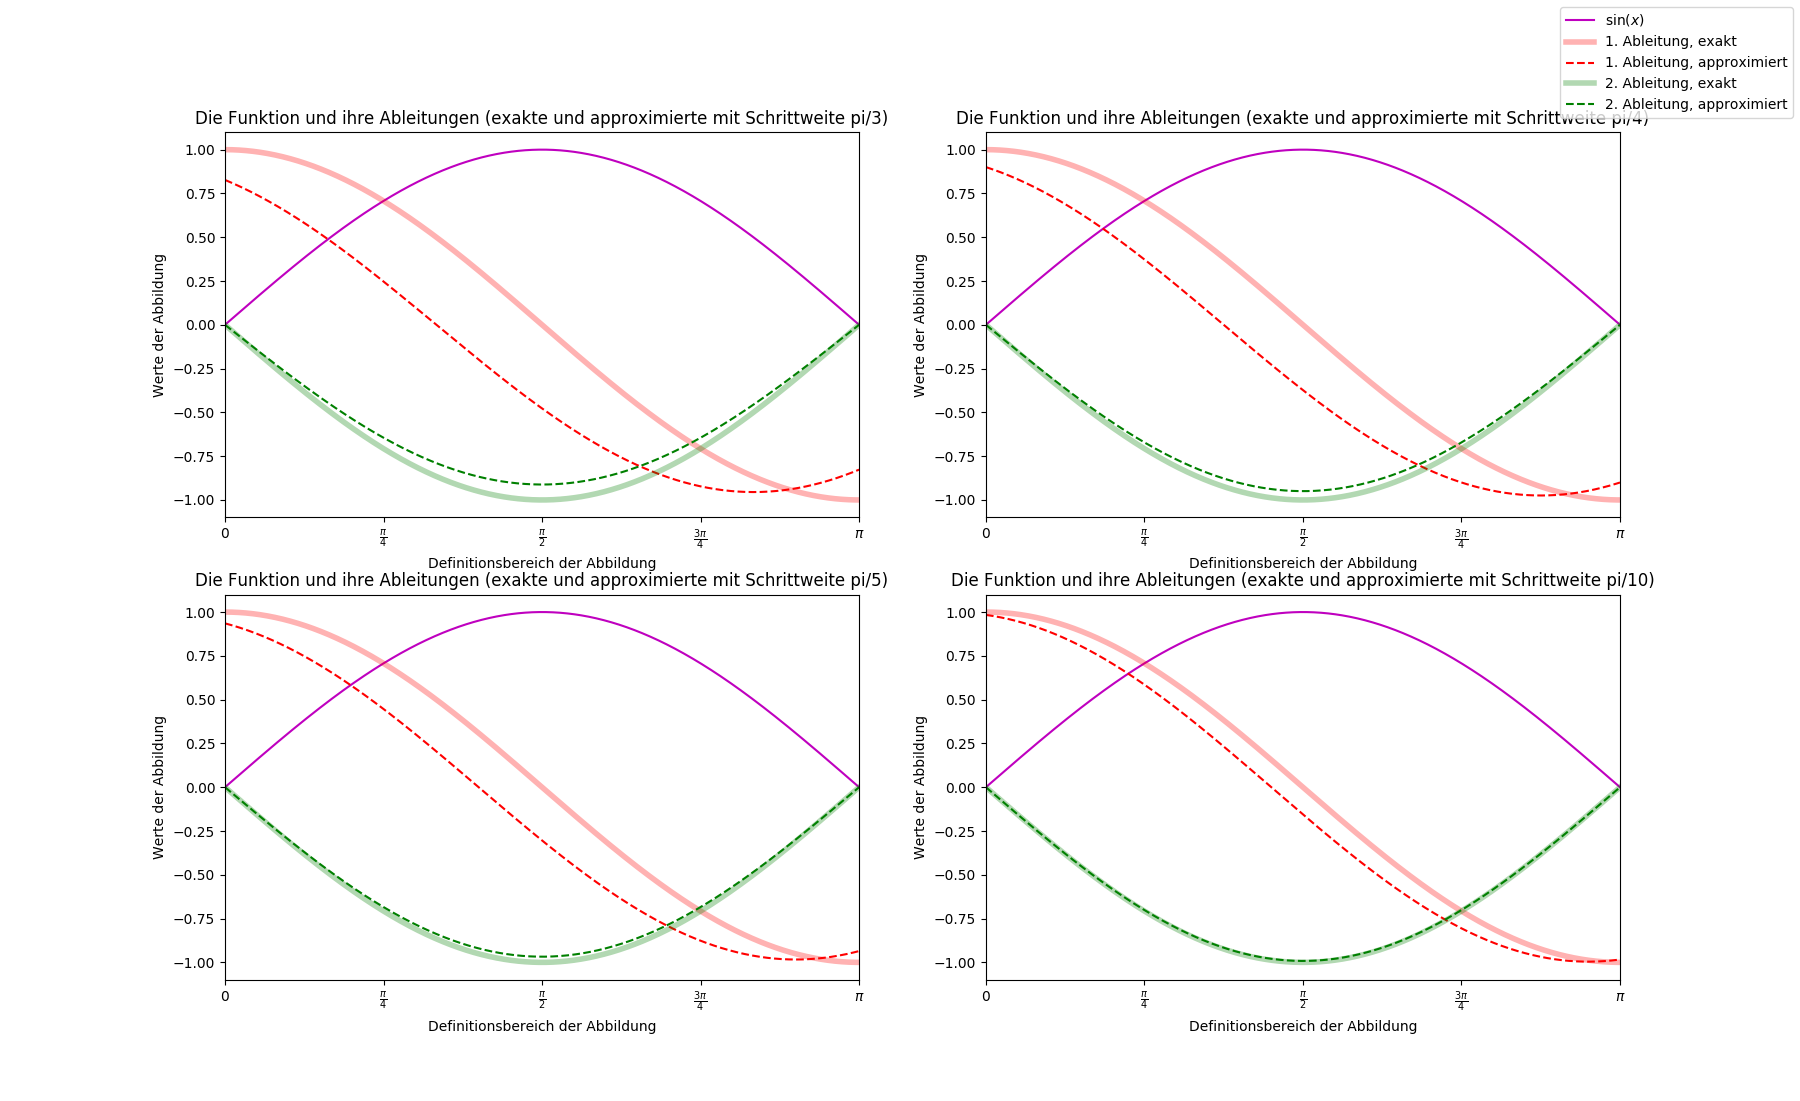
\includegraphics[width=\linewidth]{4Bilder.png}
	\caption{Die approximierten Ableitungen für verschiedene Schrittweiten.}
	\label{Abbildung 1}
\end{figure}

%%% END OF DOCUMENT %%%%%%%%%%%%%%%%%%%%%%%%%%%%%%%%%%%%%%%%%%%%%%%%%%%%%%%%%%%
\end{document}
